% LINEAR SYSTEMS AND CONTROL
% Homework 3 : 

\documentclass[10pt,a4paper]{article}
\usepackage[latin1]{inputenc}
\usepackage{amsmath}
\usepackage{amsfonts}
\usepackage{amssymb}
\usepackage{graphics} 
\usepackage{graphicx}
\usepackage{float}
\usepackage{subfigure}
\usepackage{mathtools}

\usepackage{trfsigns}
\author{Ana Huaman}
\title{\textbf{Linear Controls Homework} \\ ROB7785}
\date{}
\begin{document}
\maketitle

In class we studied the world's simplest robot, namely

\[ \ddot{p} = u \]

where $p$ is the position of the robot. If we want to include a linear friction term in the models, we would instead get

\[ \ddot{p} = -fp + u \]

where $f > 0$ is a friction coefficient

%%%%%%%%%%%%%%%%%%%%%%%%%%%%%%%%%%%%%%%%%
% Question 1
%%%%%%%%%%%%%%%%%%%%%%%%%%%%%%%%%%%%%%%%%
\section*{1.}
Under the assumption that $y = p$, produce a linear state space model of this system.

\subsection*{Solution}
We start by defining our states:

\[ 
\begin{matrix*}[l]
x_{1} = p \\
x_{2} = \dot{p}
\end{matrix*} 
\]

Then,using the equations given, we have:

\[
\begin{bmatrix}
\dot{x}_{1} \\
\dot{x}_{2}
\end{bmatrix}
=
\begin{bmatrix}
0 & 1 \\
-f & 0
\end{bmatrix}
\begin{bmatrix}
x_{1} \\
x_{2}
\end{bmatrix}
+
\begin{bmatrix}
0 \\
1
\end{bmatrix}
u
\]
% Output
\[ y = 
\begin{bmatrix}
1 & 0
\end{bmatrix}
\begin{bmatrix}
x_{1} \\
x_{2}
\end{bmatrix}
\]

Writing it shortly:
\begin{center}
\fbox{$\dot{x} =
\begin{bmatrix}
0 & 1 \\
-f & 0
\end{bmatrix}
x
+
\begin{bmatrix}
0 \\
1
\end{bmatrix}
u$}
\medskip

% Output
\fbox{ $y = 
\begin{bmatrix}
1 & 0
\end{bmatrix}
x$}
\end{center}

%%%%%%%%%%%%%%%%%%%%%%%%%%%%%%%%%%%%%%%%%
% Question 2
%%%%%%%%%%%%%%%%%%%%%%%%%%%%%%%%%%%%%%%%%
\section*{2.}
Design a state feedback controller $u = -Kx$ such that the closed-loop system has both its eigenvalues in $-\tau$, where $\tau > 0$

\subsection*{Solution}
From our system above:

\[
\dot{x} =
\begin{bmatrix}
0 & 1 \\
-f & 0
\end{bmatrix}
x
+
\begin{bmatrix}
0 \\
1
\end{bmatrix}
u
\]

Replacing $u = -Kx$

\[
\dot{x} =
\begin{bmatrix}
0 & 1 \\
-f & 0
\end{bmatrix}
x
-
\begin{bmatrix}
0 \\
1
\end{bmatrix}
\begin{bmatrix}
K_{1} & K_{2}
\end{bmatrix}
x
\]

\[
\dot{x} =
\begin{bmatrix}
0 & 1 \\
-f-K_{1} & -K_{2}
\end{bmatrix}
x \]

Finding the characteristic equation from the system above ($A-BK$)

\[ \mathcal{X}_{A-BK} =  \left | 
\begin{matrix}
\lambda & -1 \\
f + K_{1} & \lambda + K_{2}
\end{matrix}
\right | 
\]

\begin{equation} 
\mathcal{X}_{A-BK} =
\lambda^{2} + K_{2}\lambda + (f + K_{1})
\label{Eq:P1-ABK}
\end{equation}

Now, we want to have the poles: $-\tau, -\tau$. For that, our characteristic equation should have the form:

\begin{equation} \mathcal{X}_{-\tau, -\tau} =
\lambda^{2} +2\tau \lambda + \tau^{2} 
\label{Eq:P1-Tau}
\end{equation}

Now we make the coefficients of (\ref{Eq:P1-ABK}) and (\ref{Eq:P1-Tau}) equal:
\[ K_{2} = 2\tau \]
\[ f + K_{1} = \tau^{2} \]

So finally our state-feedback controller $K = \begin{bmatrix}K_{1} & K_{2}\end{bmatrix}$ is:

\begin{center}
\fbox{$K =
\begin{bmatrix}
\tau^{2} - f & 2\tau
\end{bmatrix}$}
\end{center}

%%%%%%%%%%%%%%%%%%%%%%%%%%%%%%%%%%%%%%%%%
% Question 3
%%%%%%%%%%%%%%%%%%%%%%%%%%%%%%%%%%%%%%%%%
\section*{3.}
Design an observer for this system such that the estimation error dynamics has both its eigenvalues in $-10\tau$

\subsection*{Solution}
The estimator error dynamics is given by:

\[ \dot{e} = (A-LC)e \]

where:

\[A = 
\begin{bmatrix}
0 & 1 \\
-f & 0
\end{bmatrix}
\]

\[
C =
\begin{bmatrix}
1 & 0 \end{bmatrix}
\]

and 
\[
L = 
\begin{bmatrix}L_{1} \\ L_{2} \end{bmatrix}
\]
is what we wish to design. So, as usual let's find the characteristic matrix for $(A-LC)$:

\[ A-LC = 
\begin{bmatrix}
0 & 1 \\ 
-f & 0 
\end{bmatrix}
-
\begin{bmatrix}L_{1} \\ L_{2} \end{bmatrix}
\begin{bmatrix}1 & 0 \end{bmatrix}
\] 
 
\[ A-LC = 
\begin{bmatrix}
-L_{1} & 1 \\ 
-f-L_{2} & 0 
\end{bmatrix}
\]  

Now, finding the characteristic equation:

\[ \mathcal{X}_{A-LC} =  \left | 
\begin{matrix}
\lambda + L_{1} & -1\\
f + L_{2} & \lambda 
\end{matrix}
\right | 
\]

\begin{equation} 
\mathcal{X}_{A-LC} =
\lambda^{2} + L_{1}\lambda + (f + L_{2})
\label{Eq:P3-ALC}
\end{equation}

Since we want our poles to be $-10\tau,-10\tau$, we need our equation to have the form:

\begin{equation} \mathcal{X}_{-10\tau, -10\tau} =
\lambda^{2} +20\tau \lambda + 100\tau^{2} 
\label{Eq:P3-Tau}
\end{equation}

Making the coefficients of (\ref{Eq:P3-ALC}) and (\ref{Eq:P3-Tau}) equal:

\[ L_{1} = 20\tau \]
\[ f + L_{2} = 100\tau^{2} \]

So finally our observer $L$ will be:

\begin{center}
\fbox{$L =
\begin{bmatrix}
20\tau \\
100\tau^{2} - f 
\end{bmatrix}$}
\end{center}

 
%%%%%%%%%%%%%%%%%%%%%%%%%%%%%%%%%%%%%%%%%
% Question 4-5
%%%%%%%%%%%%%%%%%%%%%%%%%%%%%%%%%%%%%%%%%
\section*{4-5}
Go to TSquare/Resources/Controls and download helicopter.m and open it up in MatLab. What you need to do in this problem is design state controllers and observers for this large system such that certain performance constraints are met.


%%%%%%%%%%%%%%%%%%%%%%%%%%%%%%%%%%%%%%%%%
% Question 4
%%%%%%%%%%%%%%%%%%%%%%%%%%%%%%%%%%%%%%%%%
\section*{4.}
Is the system controllable and observable? Is the uncontrolled system stable? (the commands \textit{rank}, \textit{obsv}, \textit{eig} might come in handy)

\subsection*{Solution}
Our system has $n=8$ ( $A_{8 \times 8}$, $B_{8 \times 4}$, $C_{6 \times 8}$ ). Let's find its main characteristics:

\begin{itemize} 
\item{\textit{Stability:} For this we find the eigenvalues of the uncontrolled system $A$:
\[ eig(A) = \begin{bmatrix} 
  -11.49675 \\ 
  -2.30362 \\
   0.23420 +  0.55126i \\
   0.23420 - 0.55126i \\ 
  -0.15932 +  0.59898i \\
  -0.15932 - 0.59898i \\
  -0.71036 \\ 
  -0.29233
  \end{bmatrix} \]

We see that we have two eigenvalues with their real part in the right side( $0.23420 \pm 0.55126i$), so:
\begin{center}
\fbox{ The uncontrolled system is NOT stable}   
\end{center}
}
\item{\textit{Controllability:} We simply calculate the Controllability matrix $\Gamma$ and check its rank:
\[ rank(\Gamma) = 8 \]
Since $rank(\Gamma) = n = 8$: 

\begin{center}
\fbox{ Our system is Completely Controllable }   
\end{center} }

\item{\textit{Observability:} Now we calculate the Observability matrix $\Omega$ and check its rank:
\[ rank(\Omega) = 8 \]
Since $rank(\Omega) = n = 8$: 
\begin{center}
\fbox{ Our system is Completely Observable }   
\end{center} }
\end{itemize}
%%%%%%%%%%%%%%%%%%%%%%%%%%%%%%%%%%%%%%%%%
% Question 5
%%%%%%%%%%%%%%%%%%%%%%%%%%%%%%%%%%%%%%%%%
\section*{5.}
Using the matlab command \textit{place}, place the observer and controller eigenvalues in such a way that $ \| x \| \leq 1 $ before $t = 3$. At the same time, we need that $ \| u \| < 50$ all the time (Note, \textit{place} does not allow for all closed-loop eigenvalues to have the same value)

\subsection*{Solution}
After some tweaking here and there I settled on these set of poles:

\[ P_{Controller} = \{-1.7, -2.1, -1.8 \pm i ,-2.0 \pm 0.5i,-2.2 \pm i \} \]
\[ P_{Observer} = \{-6.8, -8.4, -7.2 \pm 4i ,-8.0 \pm 2i,-8.8 \pm 4i \} \]

Observe that the poles for the Observer are four times faster than for the controller. Anyway, here the plots. As we may see, we keep the requirements that  $ \| x \| \leq 1 $ before $t = 3$ and $ \| u \| < 50$

	\begin{figure}[H]
			\centering
			  \subfigure[$x(t)$ vs $t$]{
			  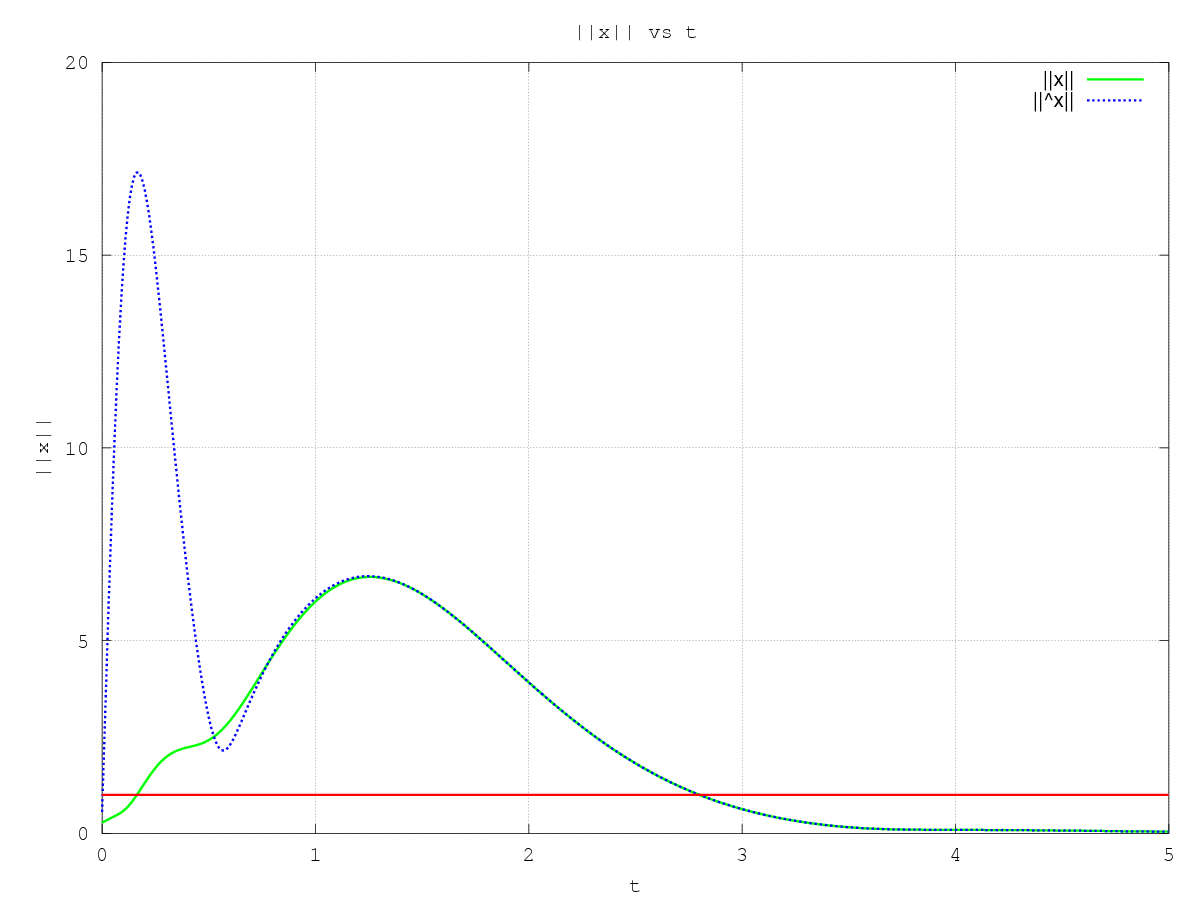
\includegraphics[scale=0.4]{figures/Question5x.png} 
	          \label{fig:Q5-x}
              }
              \subfigure[$u(t)$ vs $t$]{
	          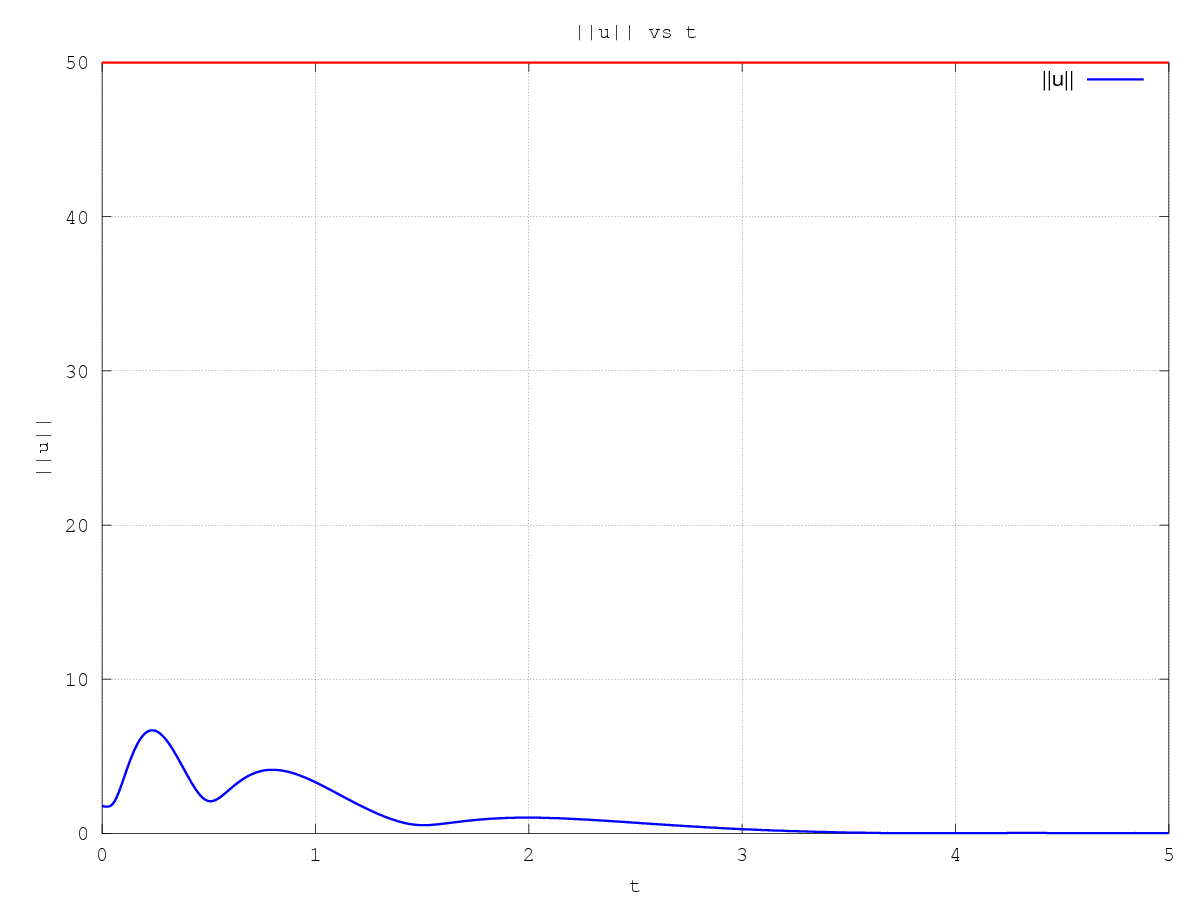
\includegraphics[scale=0.4]{figures/Question5u.png} 	
	          \label{fig:Q5-u}
              }
            \caption{Results after doing pole placement}
            \label{fig:Q5-xu}
	\end{figure}

And here are the $K$ and $L$ for the Controller and Observer respectively (by using pole placement and the poles mentioned above):

\[ K =
\begin{bmatrix}
   0.58552 & -0.76562 & -0.15151 &  0.19520 & -1.6095 &  0.013020 &  0.020439 & -0.49547 \\
   11.524 & -2.8422 &  1.4693 &  4.4342 & -0.64895 & -0.081658 & -0.21407 & -0.11119 \\
  -4.9273 & -9.1953 &  1.5847 & -0.17379 & -0.88572 &  0.12271 & -0.27671 & -0.064336 \\
  -0.29922 & -1.5976 &  0.53275 & -0.094997 & -3.9041 &  0.0087200 & -0.044122 & -0.29432
\end{bmatrix} \]

\[ L =
\begin{bmatrix}
   -11.92391 &    2.42032 &    9.40184 &   -7.69068 &    2.30093 &  -18.20559 \\
   -16.51712 &   -7.21048 &   20.63286 &  -10.52198 &    5.66922 &  -22.53554 \\
    10.14887 &    3.31190 &   -3.80115 &    6.47895 &    2.32133 &   15.86406 \\
     0.38684 &    2.91396 &   -1.74849 &   -0.15746 &   -1.26368 &    5.46524 \\
     4.87976 &    2.42736 &   -3.39559 &   10.64605 &   -3.33004 &    6.40585 \\
   178.69874 &  226.62224 &   37.52089 &   63.98300 &  121.57232 &  736.08965 \\
     9.01677 &  246.45376 &  -96.92872 &  -48.89539 & -621.59261 &  100.30267 \\ 
     4.07365 &   25.83971 &   -2.26116 &    0.93034 &  -24.48182 &   48.11639
\end{bmatrix} \]


\end{document}